%!TEX root = da2020-01.tex

\Chapter{1}{Warm-Up}

\noindent
We will start this course with an informal introduction to distributed algorithms. We will formalize the model of computing later but for now the intuitive idea of computers that can exchange messages with each others is sufficient.

\section{Running Example: Coloring Paths}

Imagine that we have $n$ computers (or \emph{nodes} as they are usually called) that are connected to each other with communication channels so that the network topology is a \emph{path}:
\begin{center}
    \includegraphics[page=\PIntroTopo]{figs.pdf}
\end{center}
The computers can exchange messages with their neighbors. All computers run the \emph{same} algorithm\mydash this is the \emph{distributed algorithm} that we will design. The algorithm will decide what messages a computer sends in each step, how it processes the messages that it receives, when it stops, and what it outputs when it stops.

In this example, the task is to find a proper \emph{coloring} of the path with $3$ colors. That is, each node has to output one of the colors, $1$, $2$, or $3$, so that neighbors have different colors\mydash here is an example of a proper solution:
\begin{center}
    \includegraphics[page=\PIntroCol]{figs.pdf}
\end{center}

\section{Challenges of Distributed Algorithm}\label{sec:intro-challenges}

With a bird's-eye view of the entire network, coloring a path looks like a very simple task: just start from one endpoint and assign colors $1$ and $2$ alternately. However, in a real-world computer network we usually do not have all-powerful entities that know everything about the network and can directly tell each computer what to do.

Indeed, when we start a networked computer, it is typically only aware of itself and the communication channels that it can use. In our simple example, the endpoints of the path know that they have one neighbor:
\begin{center}
    \includegraphics[page=\PIntroDegOne]{figs.pdf}
\end{center}
All other nodes along the path just know that they have two neighbors:
\begin{center}
    \includegraphics[page=\PIntroDegTwo]{figs.pdf}
\end{center}
For example, the second node along the path looks no different from the third node, yet somehow they have to produce \emph{different} outputs.

Obviously, the nodes have to exchange \emph{messages} with each other in order to figure out a proper solution. Yet this turns out to be surprisingly difficult even in the case of just $n = 2$ nodes:
\begin{center}
    \includegraphics[page=\PIntroTwo]{figs.pdf}
\end{center}
If we have two \emph{identical} computers connected to each other with a single communication link, both computers are started simultaneously, and both of them run the same deterministic algorithm, how could they ever end up in \emph{different} states?

The answer is that it is not possible, without some additional assumptions. In practice, we could try to rely on some real-world imperfections (e.g., the computers are seldom perfectly synchronized), but in the theory of distributed algorithms we often assume that there is some \emph{explicit} way to \emph{break symmetry} between otherwise identical computers. In this chapter, we will have a brief look at two common assumption:
\begin{itemize}[noitemsep]
    \item each computer has a unique name,
    \item each computer has a source of random bits.
\end{itemize}
In subsequent chapters we will then formalize these models, and develop a theory that will help us understand precisely what kind of tasks can be solved in each case, and how fast.


\section{Coloring with Unique Identifiers}\label{sec:algo-p3c}

There are plenty of examples of real-world networks with globally unique identifiers: public IPv4 and IPv6 addresses are globally unique identifiers of Internet hosts, devices connected to an Ethernet network have globally unique MAC addresses, mobile phones have their IMEI numbers, etc. The common theme is that the identifiers are globally unique, and the numbers can be interpreted as natural numbers:
\begin{center}
    \includegraphics[page=\PIntroId]{figs.pdf}
\end{center}
With the help of unique identifiers, it is now easy to design an algorithm that colors a path. Indeed, the unique identifiers already form a coloring with a large number of colors! All that we need to do is to reduce the number of colors to $3$.

We can use the following simple strategy. In each step, a node is active if it is a ``local maximum'', i.e., its current color is larger than the current colors of its neighbors:
\begin{center}
    \includegraphics[page=\PIntroIdA]{figs.pdf}
\end{center}
The active nodes will then pick a new color from the color palette $\{1,2,3\}$, so that it does not conflict with the current colors of their neighbors. This is always possible, as each node in a path has at most $2$ neighbors, and we have $3$ colors in our color palette:
\begin{center}
    \includegraphics[page=\PIntroIdAA]{figs.pdf}
\end{center}
Then we simply repeat the same procedure until all nodes have small colors. First find the local maxima:
\begin{center}
    \includegraphics[page=\PIntroIdB]{figs.pdf}
\end{center}
And then recolor the local maxima with colors from $\{1,2,3\}$:
\begin{center}
    \includegraphics[page=\PIntroIdBB]{figs.pdf}
\end{center}
Continuing this way we will eventually have a path that is properly colored with colors $\{1,2,3\}$:
\begin{center}
    \includegraphics[page=\PIntroIdC]{figs.pdf}\\
    \includegraphics[page=\PIntroIdCC]{figs.pdf}\\
    \includegraphics[page=\PIntroIdD]{figs.pdf}\\
    \includegraphics[page=\PIntroIdDD]{figs.pdf}\\
    \includegraphics[page=\PIntroIdE]{figs.pdf}\\
    \includegraphics[page=\PIntroIdEE]{figs.pdf}
\end{center}
Note that we may indeed be forced to use all three colors.

So far we have sketched an algorithm idea, but we still have to show that we can actually implement this idea as a distributed algorithm. Remember that there is no central control; nobody has a bird's-eye view of the entire network. Each node is an independent computer, and all computers are running the \emph{same} algorithm. What would the algorithm look like?

Let us fix some notation. Each node maintains a variable $c$ that contains its current color. Initially, $c$ is equal to the unique identifier of the node. Then computation proceeds as shown in Table~\ref{tab:algo-p3c}.

\begin{table}
    \raggedright
    \algtoprule
    \begin{descriptionb}
        \item[Repeat forever:] \mbox{}
        \begin{itemize}
            \item Send message $c$ to all neighbors.
            \item Receive messages from all neighbors. \\
                  Let $M$ be the set of messages received.
            \item If $c \notin \{1,2,3\}$ and $c > \max M$: \\
                  Let $c \gets \min\,(\{1,2,3\} \setminus M)$.
        \end{itemize}
    \end{descriptionb}
    \algbottomrule
    \caption{A simple $3$-coloring algorithm for paths.}\label{tab:algo-p3c}
\end{table}

This shows a typical structure of a distributed algorithm: an infinite send--receive--compute loop. A computer is seen as a state machine; here $c$ is the variable that holds the current state of the computer. In this algorithm, we have three \emph{stopping states}: $c = 1$, $c = 2$, and $c = 3$. It is easy to verify that the algorithm is indeed correct in the following sense:
\begin{enumerate}
    \item In any path graph, for any assignment of unique identifiers, all computers will eventually reach a stopping state.
    \item Once a computer reaches a stopping state, it never changes its state.
\end{enumerate}
The second property is very important: each computer has to know when it is safe to announce its output and stop.

Our algorithm may look a bit strange in the sense that computers that have ``stopped'' are still sending messages. However, it is fairly straightforward to rewrite the algorithm so that you could actually turn off computers that have stopped. The basic idea is that nodes that are going to switch to a stopping state first inform their neighbors about this. Each node will memorize which of its neighbors have already stopped and what were their final colors. Implementing this idea is left as Exercise~\ref{ex:intro-stopped}, and you will later see that this can be done for \emph{any} distributed algorithm. Hence, without loss of generality, we can play by the following simple rules:
\begin{itemize}
    \item The nodes are state machines that repeatedly send messages to their neighbors, receive messages from their neighbors, and update their state\mydash all nodes perform these steps synchronously in parallel.
    \item Some of the states are stopping states, and once a node reaches a stopping state, it no longer changes its state.
    \item Eventually all nodes have to reach stopping states, and these states must form a correct solution to the problem that we want to solve.
\end{itemize}
Note that here a ``state machine'' does not necessarily refer to a \emph{finite}-state machine. We can perfectly well have a state machine with infinitely many states. Indeed, in the example of Table~\ref{tab:algo-p3c} the set of possible states was the set of all positive integers.


\section{Faster Coloring with Unique Identifiers}\label{sec:algo-p3cbit}

So far we have seen that with the help of unique identifiers, it is \emph{possible} to find a $3$-coloring of a path. However, the algorithm that we designed is not particularly efficient in the worst case. To see this, consider a path in which the unique identifiers happen to be assigned in an increasing order:
\begin{center}
    \includegraphics[page=\PIntroIdBad]{figs.pdf}
\end{center}
In such a graph, in each round there is only one node that is active. In total, it will take $\Theta(n)$ rounds until all nodes have stopped.

However, it is possible to color paths \emph{much} faster. The algorithm is easier to explain if we have a \emph{directed} path:
\begin{center}
    \includegraphics[page=\PIntroIdDir]{figs.pdf}
\end{center}
That is, we have a consistent orientation in the path so that each node has at most one ``predecessor'' and at most one ``successor''. The orientations are just additional information that we will use in algorithm design\mydash nodes can always exchange information along each edge in either direction. Once we have presented the algorithm for directed paths, we will then generalize it to undirected paths in Exercise~\ref{ex:intro-undir-path}.


\subsection{Algorithm Overview}

For the sake of concreteness, let us assume that the nodes are labeled with $128$-bit unique identifiers\mydash for example, IPv6 addresses. In most real-world networks $2^{128}$ identifiers is certainly more than enough, but the same idea can be easily generalized to arbitrarily large identifiers if needed.

Again, we will interpret the unique identifiers as colors; hence our starting point is a path that is properly colored with $2^{128}$ colors. In the next section, we will present a fast color reduction algorithm for directed paths that reduces the number of colors from $2^x$ to $2x$ in one round, for any positive integer $x$. Hence in one step we can reduce the number of colors from $2^{128}$ to $2 \cdot 128 = 256$. In just four iterations we can reduce the number of colors from $2^{128}$ to $6$, as follows:
\begin{align*}
    2^{128} &\to 2 \cdot 128 = 2^8, \\
    2^8 &\to 2 \cdot 8 = 2^4, \\
    2^4 &\to 2 \cdot 4 = 2^3, \\
    2^3 &\to 2 \cdot 3 = 6.
\end{align*}
Once we have found a $6$-coloring, we can then apply the algorithm of Table~\ref{tab:algo-p3c} to reduce the number of colors from $6$ to $3$. It is easy to see that this will take at most $3$ rounds. Overall, we have an algorithm that reduces the number of colors from $2^{128}$ to $3$ in only $7$ rounds\mydash no matter how many nodes we have in the path. Compare this with the simple 3-coloring algorithm, which may take millions of rounds for paths with millions of nodes.


\subsection{Algorithm for One Step}\label{ssec:fast-color-red-one-step}

Let us now show how to reduce the number of colors from $2^x$ to $2x$ in one round; this will be achieved by doing some bit manipulations. First, each node sends its current color to its predecessor. After this step, each node $u$ knows two values:
\begin{itemize}[noitemsep]
    \item $c_0(u)$, the current color of the node,
    \item $c_1(u)$, the current color of its successor.
\end{itemize}
If a node does not have any successor, it just proceeds \emph{as if} it had a successor of some color different from $c_0(u)$.

We can interpret both $c_0(u)$ and $c_1(u)$ as $x$-bit binary strings that represent integers from range $0$ to $2^x-1$. We know that the current color of node $u$ is different from the current color of its successor, i.e., $c_0(u) \ne c_1(u)$. Hence in the two binary strings $c_0(u)$ and $c_1(u)$ there is at least one bit that differs. Define:
\begin{itemize}
    \item $i(u) \in \{0,1,\dotsc,x-1\}$ is the \emph{\textbf{index}} of the first bit that differs between $c_0(u)$ and $c_1(u)$,
    \item $b(u) \in \{0,1\}$ is the \emph{\textbf{value}} of bit number $i(u)$ in $c_0(u)$.
\end{itemize}
Finally, node $u$ chooses
\[
    c(u) = 2i(u) + b(u)
\]
as its new color.


\begin{table}
    \newcommand{\hl}[1]{\mathbf{\color{hlcolor}#1}}
    \newcommand{\node}{\raisebox{-1pt}{$\bigcirc$}}
    \newcommand{\mylf}{\\[-2pt]}
    \center
    \begin{tabular}{@{}c@{\qquad}ccccc@{}}
    \toprule
    node & input &&&& output \\
    $u$ & $c_0(u)$ & $c_1(u)$ & $i(u)$ & $b(u)$ & $c(u)$ \\
    \midrule
    $\cdots$ & $\cdots$ & $\cdots$ & $\cdots$ & $\cdots$ & $\cdots$ \mylf
    $\downarrow$ \mylf
    \node & $01111\hl{0}11_2$ & $00101\hl{1}11_2$ & $2$ & $0$ & $4$ \mylf
    $\downarrow$ \mylf
    \node & $00101\hl{1}11_2$ & $01101\hl{0}11_2$ & $2$ & $1$ & $5$ \mylf
    $\downarrow$ \mylf
    $\node$ & $01101011_2$ & $\cdots$ & $\cdots$ & $\cdots$ & $\cdots$ \mylf
    $\downarrow$ \mylf
    $\cdots$ & $\cdots$ \mylf
    \midrule
    $\cdots$ & $\cdots$ & $\cdots$ & $\cdots$ & $\cdots$ & $\cdots$ \mylf
    $\downarrow$ \mylf
    \node & $01111\hl{0}11_2$ & $00101\hl{1}11_2$ & $2$ & $0$ & $4$ \mylf
    $\downarrow$ \mylf
    \node & $0\hl{0}101111_2$ & $0\hl{1}101111_2$ & $6$ & $0$ & $12$ \mylf
    $\downarrow$ \mylf
    $\node$ & $01101111_2$ & $\cdots$ & $\cdots$ & $\cdots$ & $\cdots$ \mylf
    $\downarrow$ \mylf
    $\cdots$ & $\cdots$ \mylf
    \bottomrule
    \end{tabular}
    \caption{Fast color reduction algorithm for directed paths: reducing the number of colors from $2^x$ to $2x$, for $x = 8$. There are two interesting cases: either $i(u)$ is the same for two neighbors (first example), or they are different (second example). In the first case, the values $b(u)$ will differ, and in the second case, the values $i(u)$ will differ. In both cases, the final colors $c(u)$ will be different.}\label{tab:algo-p3cbit}
\end{table}


\subsection{An Example}

Let $x = 8$, i.e., nodes are colored with $8$-bit numbers. Assume that we have a node $u$ of color $123$, and $u$ has a successor $v$ of color $47$; see Table~\ref{tab:algo-p3cbit} for an illustration. In binary, we have
\begin{align*}
    c_0(u) &= 01111011_2, \\
    c_1(u) &= 00101111_2.
\end{align*}
\begin{samepage}
Counting from the least significant bit, node $u$ can see that:
\begin{itemize}[noitemsep]
    \item bit number $0$ is the same in both $c_0(u)$ and $c_1(u)$,
    \item bit number $1$ is the same in both $c_0(u)$ and $c_1(u)$,
    \item bit number $2$ is different in $c_0(u)$ and $c_1(u)$.
\end{itemize}
\end{samepage}
Hence we will set
\[
    i(u) = 2, \quad
    b(u) = 0, \quad
    c(u) = 2\cdot2 + 0 = 4.
\]
That is, node $u$ picks $4$ as its new color. If all other nodes run the same algorithm, this will be a valid choice\mydash as we will argue next, both the predecessor and the successor of $u$ will pick a color that is different from~$4$.


\subsection{Correctness}

Clearly, the value $c(u)$ is in the range $\{0,1,\dotsc,2x-1\}$. However, it is not entirely obvious that these values actually produce a proper $2x$-coloring of the path. To see this, consider a pair of nodes $u$ and $v$ so that $v$ is the successor of $u$. By definition, $c_1(u) = c_0(v)$. We need to show that $c(u) \ne c(v)$. There are two cases\mydash see Table~\ref{tab:algo-p3cbit} for an example:
\begin{enumerate}
    \item $i(u) = i(v) = i$: We know that $b(u)$ is bit number $i$ of $c_0(u)$, and $b(v)$ is bit number $i$ of $c_1(u)$. By the definition of $i(u)$, we also know that these bits differ. Hence $b(u) \ne b(v)$ and $c(u) \ne c(v)$.
    \item $i(u) \ne i(v)$: No matter how we choose $b(u) \in \{0,1\}$ and $b(v) \in \{0,1\}$, we have $c(u) \ne c(v)$.
\end{enumerate}
We have argued that $c(u) \ne c(v)$ for any pair of two adjacent nodes $u$ and $v$, and the value of $c(u)$ is an integer between $0$ and $2x-1$ for each node $u$. Hence the algorithm finds a proper $2x$-coloring in one round.


\subsection{Iteration}

The algorithm that we presented in this section can reduce the number of colors from $2^x$ to $2x$ in one round; put otherwise, we can reduce the number of colors from $x$ to $O(\log x)$ in one round.

If we iterate the algorithm, we can reduce the number of colors from $x$ to $6$ in $O(\log^* x)$ rounds (please refer to Section~\ref{sec:intro-app} for the definition of the $\log^*$ function if you are not familiar with it).

Once we have reduced the number of colors to $6$, we can use the simple color reduction algorithm from Section~\ref{sec:algo-p3c} to reduce the number of colors from $6$ to $3$ in $3$ rounds. The details of the analysis are left as Exercises \ref{ex:logstar} and~\ref{ex:logstar-tight}.


\section{Coloring with Randomized Algorithms}\label{sec:algo-p3crand}

So far we have used unique identifiers to break symmetry. Another possibility is to use randomness. Here is a simple randomized distributed algorithm that finds a proper $3$-coloring of a path: nodes try to pick colors from the palette $\{1,2,3\}$ uniformly at random, and they stop once they succeed in picking a color that is different from the colors of their neighbors.


\subsection{Algorithm}

Let us formalize the \emph{simple randomized 3-coloring algorithm} that we sketched above. Each node $u$ has a flag $s(u) \in \{0,1\}$ indicating whether it has stopped, and a variable $c(u) \in \{1,2,3\}$ that stores its current color. If $s(u) = 1$, a node has stopped and its output is $c(u)$.

In each step, each node $u$ with $s(u) = 0$ picks a new color $c(u) \in \{1,2,3\}$ uniformly at random. Then each node sends its current color $c(u)$ to its neighbors. If $c(u)$ is different from the colors of its neighbors, $u$ will set $s(u) = 1$ and stop; otherwise it tries again in the next round.


\subsection{Analysis}

It is easy to see that in each step, a node $u$ will stop with probability at least $1/3$: after all, no matter what its neighbors do, there is at least one choice for $c(u) \in \{1,2,3\}$ that does not conflict with its neighbors.

Fix a positive constant $C$. Consider what happens if we run the algorithm for
\[
    k = (C+1) \log_{3/2} n
\]
steps, where $n$ is the number of nodes in the network. Now the probability that a given node $u$ has not stopped after $k$ steps is at most
\[
    (1 - 1/3)^k = \frac{1}{n^{C+1}}.
\]
By the union bound, the probability that there is a node that has not stopped is at most $1/n^C$. Hence with probability at least $1-1/n^C$, all nodes have stopped after $k$ steps.


\subsection{With High Probability}

Let us summarize what we have achieved: for any given constant $C$, there is an algorithm that runs for $k = O(\log n)$ rounds and produces a proper $3$-coloring of a path with probability $1-1/n^C$. We say that the algorithm runs in time $O(\log n)$ \emph{with high probability}\mydash here the phrase ``high probability'' means that we can choose any constant $C$ and the algorithm will succeed at least with a probability of $1-1/n^C$. Note that even for a moderate value of $C$, say, $C = 10$, the success probability approaches $1$ very rapidly as $n$ increases.


\section{Summary}

In this chapter we have seen three different distributed algorithms for $3$-coloring paths:
\begin{itemize}
    \item A simple 3-coloring algorithm, Section~\ref{sec:algo-p3c}: A deterministic algorithm for paths with unique identifiers. Runs in $O(n)$ rounds, where $n$ is the number of nodes.
    \item A fast 3-coloring algorithm, Section~\ref{sec:algo-p3cbit}: A deterministic algorithm for \emph{directed} paths with unique identifiers. Runs in $O(\log^* x)$ rounds, where $x$ is the largest identifier.
    \item A simple randomized 3-coloring algorithm, Section~\ref{sec:algo-p3crand}: A randomized algorithm for paths without unique identifiers. Runs in $O(\log n)$ rounds with high probability.
\end{itemize}
We will explore and analyze these algorithms and their variants in more depth in the exercises.

\section{Quiz}

Construct a directed path of 3 nodes that is labeled with unique identifiers (of any size) such that the following holds: After two iterations of the fast color reduction algorithm from Section~\ref{ssec:fast-color-red-one-step}, the color of the first node is 7.

It is enough to just list the three unique identifiers (in decimal); there is no need to explain anything else.

\section{Exercises}

\begin{ex}[maximal independent sets]\label{ex:intro-mis}
    A \emph{maximal independent set} is a set of nodes $I$ that satisfies the following properties:
    \begin{itemize}[noitemsep]
        \item for each node $v \in I$, none of its neighbors are in $I$,
        \item for each node $v \notin I$, at least one of its neighbors is in $I$.
    \end{itemize}
    Here is an example\mydash the nodes labeled with a ``1'' form a maximal independent set:
    \begin{center}
        \includegraphics[page=\PIntroMis]{figs.pdf}
    \end{center}
    Your task is to design a distributed algorithm that finds a maximal independent set in any path graph, for each of the following settings:
    \begin{subex}
        \item\label{subex:intro-mis-a} a deterministic algorithm for paths with arbitrarily large unique identifiers,
        \item\label{subex:intro-mis-b} a fast deterministic algorithm for \emph{directed} paths with $128$-bit unique identifiers,
        \item\label{subex:intro-mis-c} a randomized algorithm that does not need unique identifiers. 
    \end{subex}
    In part \ref{subex:intro-mis-a}, use the techniques presented in Section~\ref{sec:algo-p3c},
    in part \ref{subex:intro-mis-b}, use the techniques presented in Section~\ref{sec:algo-p3cbit}, and
    in part \ref{subex:intro-mis-c}, use the techniques presented in Section~\ref{sec:algo-p3crand}.
\end{ex}

\begin{ex}[stopped nodes]\label{ex:intro-stopped}
    Rewrite the greedy algorithm of Table~\ref{tab:algo-p3c} so that stopped nodes do not need to send messages. Be precise: explain your algorithm in detail so that you could easily implement it.
\end{ex}

\begin{ex}[undirected paths]\label{ex:intro-undir-path}
    The fast 3-coloring algorithm from Section~\ref{sec:algo-p3cbit} finds a $3$-coloring very fast in any directed path. Design an algorithm that is almost as fast and works in any path, even if the edges are not directed. You can assume that the range of identifiers is known.

    \hint{Use the local maxima and minima to partition the path in subpaths so that within each subpath we have unique identifiers given in an increasing order. Use this ordering to orient each subpath. Then we can apply the fast color reduction algorithm in each subpath. Finally, combine the solutions.}
\end{ex}

\begin{ex}[randomized and fast]
    The simple randomized 3-coloring algorithm finds a $3$-coloring in time $O(\log n)$ with high probability, and it does not need any unique identifiers. Can you design a randomized algorithm that finds a $3$-coloring in time $o(\log n)$ with high probability? You can assume that $n$ is known.

    \hint{Design a randomized algorithm that finds a coloring with a large number of colors quickly. Then apply the technique of the fast 3-coloring algorithm from Section~\ref{sec:algo-p3cbit} to reduce the number of colors to $3$ quickly.}
\end{ex}

\begin{ex}[asymptotic analysis]\label{ex:logstar}
    Analyze the fast 3-coloring algorithm from Section~\ref{sec:algo-p3cbit}:
    \begin{subex}
        \item Assume that we are given a coloring with $x$ colors; the colors are numbers from $\{1,2,\dotsc,x\}$. Show that we can find a $3$-coloring in time $O(\log^* x)$.
        \item Assume that we are given unique identifiers that are polynomial in $n$, that is, there is a constant $c = O(1)$ such that the unique identifiers are a subset of $\{1,2,\dotsc,n^c\}$. Show that we can find a $3$-coloring in time $O(\log^* n)$.
    \end{subex}
\end{ex}

\begin{exs}[tight analysis]\label{ex:logstar-tight}
    Analyze the fast 3-coloring algorithm from Section~\ref{sec:algo-p3cbit}:
    Assume that we are given a coloring with $x$ colors, for any integer $x \ge 6$; the colors are numbers from $\{1,2,\dotsc,x\}$. Show that we can find a $6$-coloring in time $\log^*(x)$, and therefore a $3$-coloring in time $\log^*(x) + 3$.
    \hint{Consider the following cases separately:
    \begin{center}
    (i)~$\log^* x \le 2$,\quad
    (ii)~$\log^* x = 3$,\quad
    (iii)~$\log^* x \ge 4$.
    \end{center}
    In case~(iii), prove that after $\log^*(x)-3$ iterations, the number of colors is at most $64$.}
\end{exs}

\begin{exs}[oblivious algorithms]\label{ex:oblivious}
    The simple 3-coloring algorithm works correctly even if we do not know how many nodes there are in the network, or what is the range of unique identifiers\mydash we say that the algorithm is \emph{oblivious}. Adapt the fast 3-coloring algorithm from Section~\ref{sec:algo-p3cbit} so that it is also oblivious.
    \hint{One possible strategy is this: Choose some threshold, e.g., $d = 10$. Focus on the nodes that have identifiers smaller than $d$, and find a proper $3$-coloring in those parts, in time $O(\log^* d)$. Remove the nodes that are properly colored. Then increase threshold $d$, and repeat. Be careful with the way in which you increase $d$. Show that you can achieve a running time of $O(\log^* x)$, where $x$ is the largest identifier, without knowing $x$ in advance.}
\end{exs}


\section{Bibliographic Notes}

The fast 3-coloring algorithm (Section~\ref{sec:algo-p3cbit}) was originally presented by Cole and Vishkin~\cite{cole86deterministic} and further refined by Goldberg et al.~\cite{goldberg88parallel}; in the literature, it is commonly known as the ``Cole--Vishkin algorithm''. Exercise~\ref{ex:oblivious} was inspired by Korman et al.~\cite{korman11removing}.
